\section{Illumination de Phong}

\begin{frame}
	\frametitle{Illumination}
	\begin{block}{Comment faire?}
		Sphères affichés $\rightarrow$ gestion de la lumière qui se réfélchie sur les boules
	\end{block}
	\begin{block}{Illumination de Phong}
		\begin{enumerate}
			\item Lumière diffuse
			\item Lumière spéculaire
		\end{enumerate}
	\end{block}
\end{frame}
	
\begin{frame}
	\frametitle{Lumière diffuse}
	\begin{block}{Lumière diffuse}
		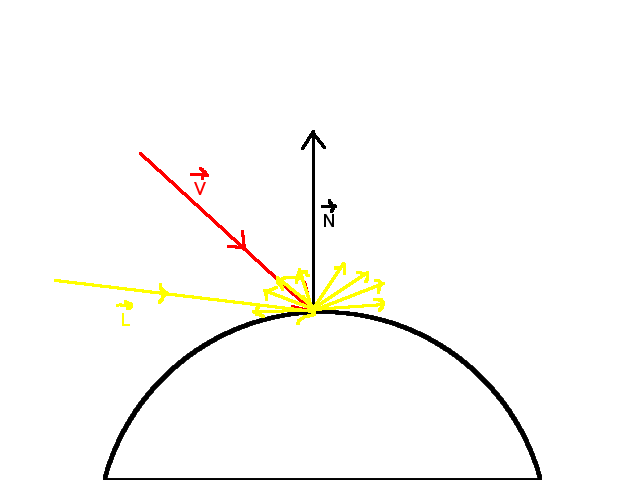
\includegraphics[width = 300px]{phong1.png} 
	\end{block}
\end{frame}
	
\begin{frame}
	\frametitle{Lumière spéculaire}
	\begin{block}{Lumière diffuse}
		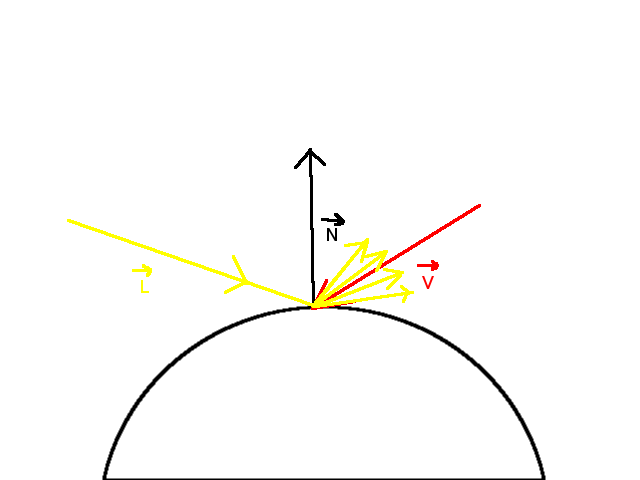
\includegraphics[width = 300px]{phong2.png} 
	\end{block}
\end{frame}

\begin{frame}
	\frametitle{Combinaison des 2}
	\begin{block}{Combinaison}
		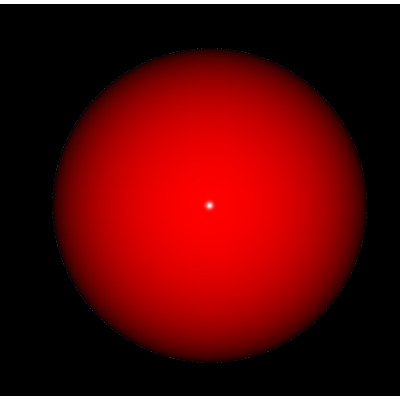
\includegraphics[width = 200px]{phong3.png} 
	\end{block}
\end{frame}

\begin{frame}
	\frametitle{Ajout de la réflexion}
	\begin{block}{Réflexion}
		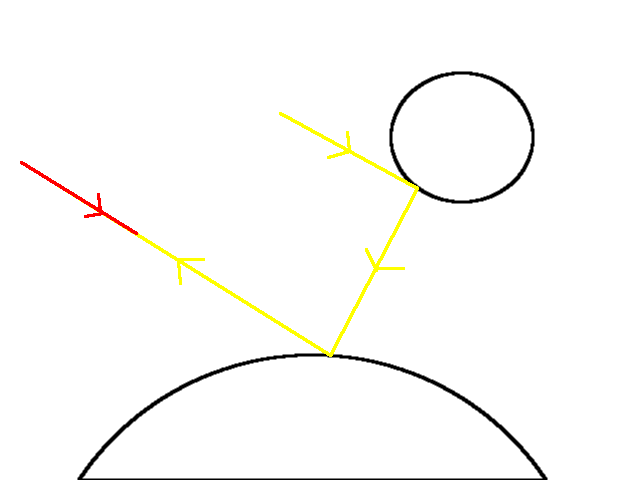
\includegraphics[width = 300px]{reflection.png} 
	\end{block}
\end{frame}

\begin{frame}
	\frametitle{Exemple de réflexion}
	\begin{block}{Exemple}
		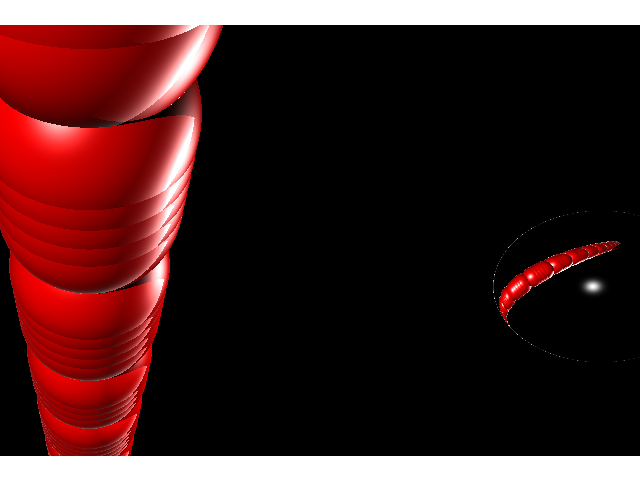
\includegraphics[width = 300px]{brillance.png} 
	\end{block}
\end{frame}

\begin{frame}
	\frametitle{Ajout de la transparence}
	\begin{block}{Transparence}
		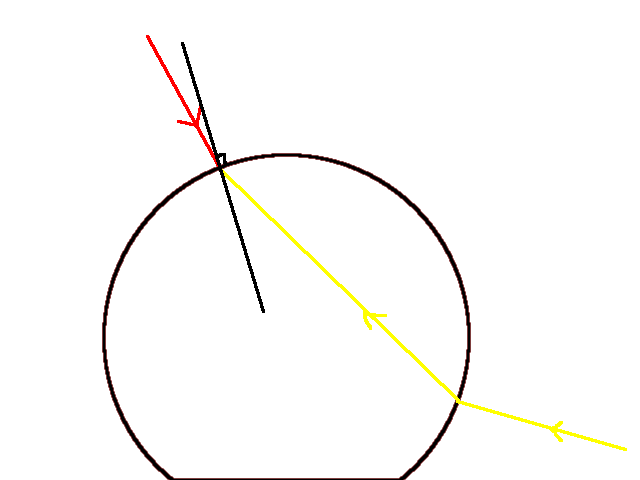
\includegraphics[width = 300px]{transparence.png} 
	\end{block}
\end{frame}

\begin{frame}
	\frametitle{Exemple de transparence}
	\begin{block}{Exemple}
		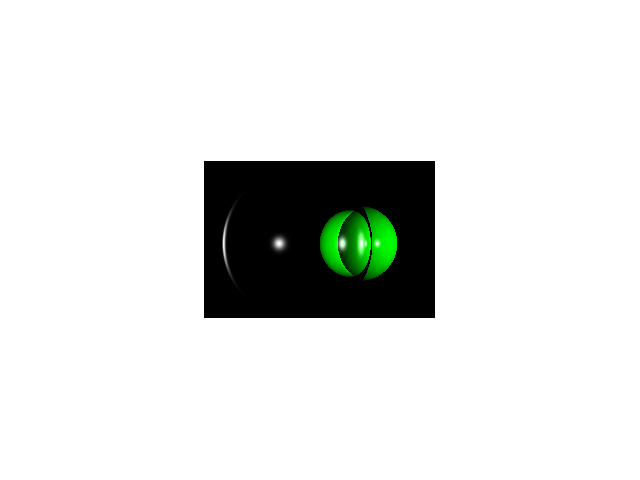
\includegraphics[width = 300px]{Untitled.png} 
	\end{block}
\end{frame}
